\documentclass[10pt,a4paper]{article}

% This standalone file is compatible with the ATAI Overleaf template.
% Copy the content into the supplied template if the course template is required.
\usepackage[margin=2.0cm]{geometry}
\usepackage[T1]{fontenc}
\usepackage{lmodern}
\usepackage{microtype}
\usepackage{enumitem}
\usepackage{xcolor}
\usepackage{booktabs}
\usepackage{float}
\usepackage{tikz}
\usetikzlibrary{arrows.meta,positioning,fit,shapes.geometric}
\usepackage[hidelinks]{hyperref}

\definecolor{ataiNavy}{HTML}{102A43}
\definecolor{ataiTeal}{HTML}{0F766E}
\definecolor{ataiLight}{HTML}{E7F6F2}
\hypersetup{colorlinks=true,linkcolor=ataiTeal,citecolor=ataiTeal,urlcolor=ataiTeal}
\setlist[itemize]{leftmargin=*,nosep}
\setlist[enumerate]{leftmargin=*,nosep}
\setlength{\parindent}{0pt}
\setlength{\parskip}{3pt}

\title{\vspace{-1.5 em}\textbf{Advanced Topics in Artificial Intelligence - Stage 2 Factual questions}}

\author{\vspace{0 em} Tristan Hein - Thi Tho Pham}
\date{\vspace{-1 em} October 2026}

\begin{document}
\maketitle
\vspace{-3 em}

\begin{abstract}
We present a natural-language factual question answering chatbot for the movie knowledge graph. The system resolves entities and relations from English questions, generates transparent SPARQL, executes it over RDFLib~\cite{rdflib}, and verbalizes the result. It extends the Stage 1 SPARQL bot while supporting typos, alternative relation directions, negation, aggregation, sorting, and simple filtering.
\end{abstract}

\section{Problem and scope}
The input is a factual question about movies, people, countries, dates, awards, or related knowledge-graph entities. Movie names do not need quotation marks. The intended questions contain identifiable entities, including small misspellings; vague descriptions are outside the scope. Answers are returned as entity labels rather than only Wikidata identifiers~\cite{wikidata}.


\section{Chatbot structure}
The chatbot has four conceptual layers. First, the interface receives a user question and manages communication with the bot service~\cite{speakeasy}. Second, the language-understanding layer identifies entities, relations, direction, and operators such as negation or counting. Third, the query layer converts this interpretation into SPARQL. Finally, the knowledge-graph layer executes the query over RDFLib and turns the returned entities into a concise natural-language answer. Separate evaluation data and test cases verify the factual examples. The interaction between the parties is shown in Figure~\ref{fig:party-relations}; the internal processing flow is shown in Figure~\ref{fig:conceptual-structure}.

\begin{center}
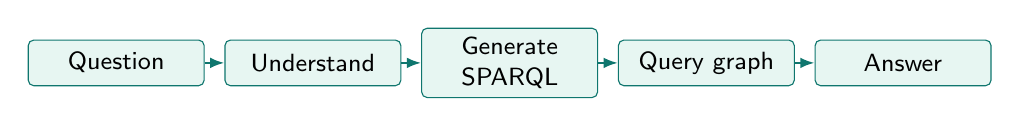
\begin{tikzpicture}[
    font=\sffamily\small,
    flowbox/.style={draw=ataiTeal, rounded corners=2pt, fill=ataiLight, align=center, minimum height=0.58cm, text width=2.0cm},
    flowarrow/.style={-{Latex[length=1.8mm]}, thick, draw=ataiTeal}
]
\node[flowbox] (f1) {Question};
\node[flowbox, right=0.25cm of f1] (f2) {Understand};
\node[flowbox, right=0.25cm of f2] (f3) {Generate SPARQL};
\node[flowbox, right=0.25cm of f3] (f4) {Query graph};
\node[flowbox, right=0.25cm of f4] (f5) {Answer};
\draw[flowarrow] (f1) -- (f2);
\draw[flowarrow] (f2) -- (f3);
\draw[flowarrow] (f3) -- (f4);
\draw[flowarrow] (f4) -- (f5);
\end{tikzpicture}
\end{center}

The reasoning component receives a message and first detects whether it is already SPARQL. Natural-language messages pass through four stages:

\begin{enumerate}
    \item \textbf{Entity resolution.} Quoted and unquoted n-grams are matched against graph labels. Normalized exact matching is attempted first, followed by conservative fuzzy matching for small typos. Common question and relation words are excluded from fuzzy entity matching.
    \item \textbf{Relation and direction detection.} Hand-written English aliases cover common movie properties such as director, screenwriter, composer, release date, country of origin, cast, and awards. Graph property labels provide additional aliases. The question form determines whether the answer is the subject or object of the relation; the reverse direction is tried when appropriate.
    \item \textbf{SPARQL construction.} The agent creates a transparent query with label matching, optional English labels, and \texttt{SELECT DISTINCT}. Counts use \texttt{COUNT}, earliest/latest questions use \texttt{ORDER BY}, and simple negation uses \texttt{FILTER NOT EXISTS}. Release-date questions without a named entity use a global date query.
    \item \textbf{Execution and verbalization.} RDFLib executes the query over \texttt{data/graph.nt}. The response keeps all ordinary results and joins their labels into a concise factual sentence. Negation and filtering results are capped at four displayed entities followed by ``...'' to avoid overwhelming the chat interface.
\end{enumerate}
\newpage
\section{Requirements}
The chatbot addresses the assignment requirements with the following techniques.

\begin{center}
\small
\begin{tabular}{@{}p{0.20\linewidth}p{0.65\linewidth}@{}}
\toprule
\textbf{Requirement} & \textbf{Technique used} \\
\midrule
No quotation marks & Generate entity n-grams from the whole question and match them against normalized \texttt{rdfs:label} values. \\
Small typos & Apply \texttt{SequenceMatcher} fuzzy matching to short candidate spans, with a confidence threshold and question-word exclusions. \\
Up to 10 answer entities & Use \texttt{SELECT DISTINCT}; collect every returned row and preserve the complete entity list for ordinary questions. \\
Forward and inverse relations & Detect answer direction from question patterns and retry the opposite subject/object direction when the preferred query has no answer. \\
Simple negation & Build a positive candidate universe and exclude linked candidates with \texttt{FILTER NOT EXISTS}. \\
Aggregation & Translate count wording such as ``how many'' into \texttt{COUNT(DISTINCT ?answer)}. \\
Sorting & Use \texttt{ORDER BY ASC/DESC(?date)} for earliest, oldest, latest, and most-recent questions. \\
Filtering & Extract simple year constraints and generate before/after/equal \texttt{YEAR(?date)} filters; entity-free release questions use a global date query. \\
\bottomrule
\end{tabular}
\end{center}

\section{Implementation and optimization}
The repository separates the chatbot into graph loading, factual QA, Speakeasy transport, tests, examples, and data directories. The graph-selection order is explicit: an optional \texttt{KNOWLEDGE\_GRAPH\_PATH}, the Nuvolos dataset, the local \texttt{data/graph.nt}, and finally the small Stage 1 graph.

The full course graph contains 2,413,825 triples. Parsing this file is the main startup cost. To reduce per-question latency, the agent builds in-memory indexes for normalized labels, label-to-entity mappings, and preferred labels. Common single-hop relations and counts use direct RDFLib lookups through these indexes instead of repeatedly scanning all labels with SPARQL. Sorting and entity-free release-date filters use the same indexed path. Generated SPARQL is still printed for debugging and reproducibility.

\section{Evaluation}
The implementation was tested with the six published Stage 2 examples: screenplay writers for The Handmaiden, countries of origin for Interstellar, the release date of Manchester by the Sea, Sofia Coppola's earliest film, awards received by There Will Be Blood, and the composer of The Father. All six examples pass against the full course graph.

Additional test cases cover the required question forms:
\begin{itemize}
    \item \emph{Entity variation:} ``Who directed The Handmaiden?'' and ``Who directed Insde Out?''
    \item \emph{Aggregation:} ``How many countries of origin does Interstellar have?''
    \item \emph{Sorting:} ``Which film directed by Christopher Nolan was released most recently?''
    \item \emph{Filtering and negation:} ``Which movies were released before 2010?'' and ``Which movies were not directed by Sofia Coppola?''
\end{itemize}

\section{Limitations and next steps}
The system is designed for the constrained factual questions rather than open-domain dialogue. A negative query depends on a meaningful candidate universe, such as movies, awards, or countries. It does not infer a universal real-world complement. Fuzzy matching is deliberately conservative to avoid turning vague descriptions into unsupported guesses. The next practical improvement would be persistent graph/index caching so that the large RDF graph does not need to be parsed and indexed after every process start.

\clearpage
\section*{System relations and conceptual code structure}
This page provides the two complementary views of the chatbot. Figure~\ref{fig:party-relations} describes how the user, messaging API, chatbot service, reasoning layer, and knowledge graph exchange information. Figure~\ref{fig:conceptual-structure} shows the internal processing sequence that converts a natural-language question into a formatted answer.

\textbf{Relations between the parties}
\begin{figure}[H]
\centering
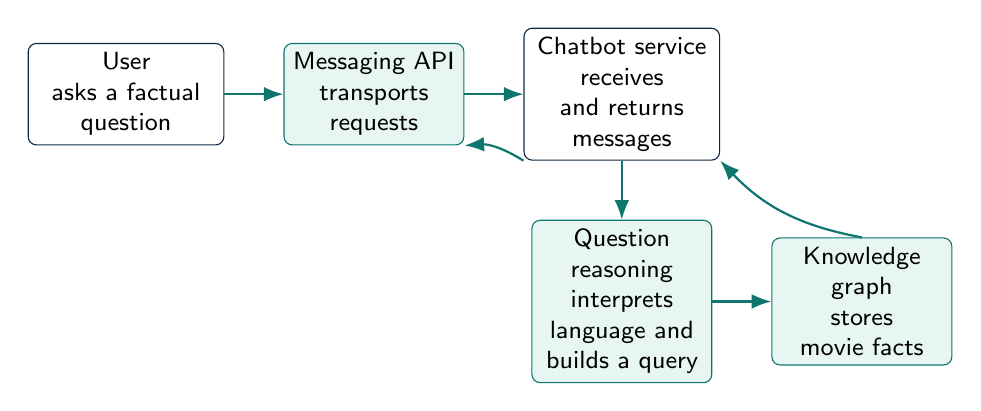
\begin{tikzpicture}[
    font=\sffamily\small,
    node distance=0.65cm and 0.75cm,
    box/.style={draw=ataiTeal, rounded corners=3pt, fill=ataiLight, align=center, minimum height=0.78cm, text width=2.05cm},
    wide/.style={draw=ataiNavy, rounded corners=3pt, fill=white, align=center, minimum height=0.78cm, text width=2.25cm},
    arrow/.style={-{Latex[length=2.5mm]}, thick, draw=ataiTeal}
]
\node[wide] (user) {User\\\small asks a factual question};
\node[box, right=of user] (api) {Messaging API\\\small transports requests};
\node[wide, right=of api] (bot) {Chatbot service\\\small receives and returns messages};
\node[box, below=0.75cm of bot] (reason) {Question reasoning\\\small interprets language and builds a query};
\node[box, right=of reason] (graph) {Knowledge graph\\\small stores movie facts};
\draw[arrow] (user) -- (api);
\draw[arrow] (api) -- (bot);
\draw[arrow] (bot) -- (reason);
\draw[arrow] (reason) -- (graph);
\draw[arrow] (bot.south west) to[bend right=18] (api.south east);
\draw[arrow] (graph.north) to[bend left=18] (bot.south east);
\end{tikzpicture}
\caption{Relationship between the user, chatbot service}
\label{fig:party-relations}
\end{figure}

\vspace{0.7em}
\textbf{Conceptual code structure}
\begin{figure}[H]
\centering
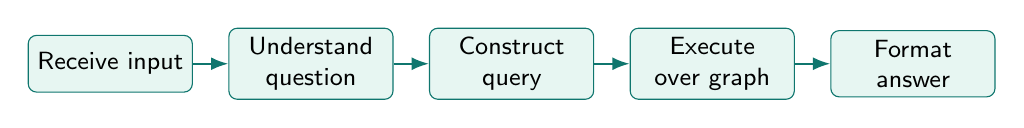
\begin{tikzpicture}[
    font=\sffamily\small,
    node distance=0.45cm and 0.45cm,
    box/.style={draw=ataiTeal, rounded corners=3pt, fill=ataiLight, align=center, minimum height=0.72cm, text width=1.85cm},
    arrow/.style={-{Latex[length=2.2mm]}, thick, draw=ataiTeal}
]
\node[box] (input2) {Receive input};
\node[box, right=of input2] (understand2) {Understand question};
\node[box, right=of understand2] (query2) {Construct query};
\node[box, right=of query2] (execute2) {Execute over graph};
\node[box, right=of execute2] (answer2) {Format answer};
\draw[arrow] (input2) -- (understand2);
\draw[arrow] (understand2) -- (query2);
\draw[arrow] (query2) -- (execute2);
\draw[arrow] (execute2) -- (answer2);
\end{tikzpicture}
\caption{Processing from input reception to answer}
\label{fig:conceptual-structure}
\end{figure}

\vspace{0.6em}
\begin{center}
\begin{tabular}{@{}ll@{}}
\toprule
\textbf{Component} & \textbf{Role} \\
\midrule
Language understanding & Entity, relation, direction, and operator detection \\
Query generation & SPARQL construction with filters, aggregation, and sorting \\
Knowledge-graph access & RDFLib loading, SPARQL execution, and result conversion \\
Evaluation layer & Published examples, smoke tests, and local fallback data \\
\bottomrule
\end{tabular}
\end{center}

\footnotesize
\begin{thebibliography}{9}
\setlength{\itemsep}{0pt}
\bibitem{wikidata}
Wikimedia Foundation, ``Wikidata: The free collaborative knowledge base,''
\url{https://www.wikidata.org/}, accessed October 2026.

\bibitem{rdflib}
RDFLib Developers, ``RDFLib: A Python library for working with RDF,''
\url{https://rdflib.readthedocs.io/}, accessed October 2026.

\bibitem{speakeasy}
University of Zurich, ``Speakeasy chatbot platform,'' course infrastructure for ATAI 2026.
\end{thebibliography}

\end{document}
